\documentclass[../main.tex]{subfiles}
\usepackage[english]{babel}
\graphicspath{{\subfix{../images}}}
\begin{document}

\section{Radiomics}

Radiomics is identified as a process, made of several steps, which aims to extract quantitative information (\textit{features}) during medical images analysis. 
Generally, it exploits the power of Machine Learning algorithms to connect features extracted from the images, with a predictive quantification of the clinical outcomes \cite{kumar2012radiomics}.
The reason behind the widespread of radiomics applications is that
mining data from intensity, size, shape or texture reveals relations between biomedical images information and the patients' pathophysiological characteristics \cite{gillies2016radiomics-more-than-images}.


\subsection{Radiomics pipeline}\label{sec:radiomic-pipeline}

The method to perform radiomic analysis is characterized by four standard steps: image acquisition, image segmentation, feature extraction and data analysis. The full procedure is shown in Figure \ref{fig:radiomics_pipeline}.

\begin{figure}[H] 
\begin{center}
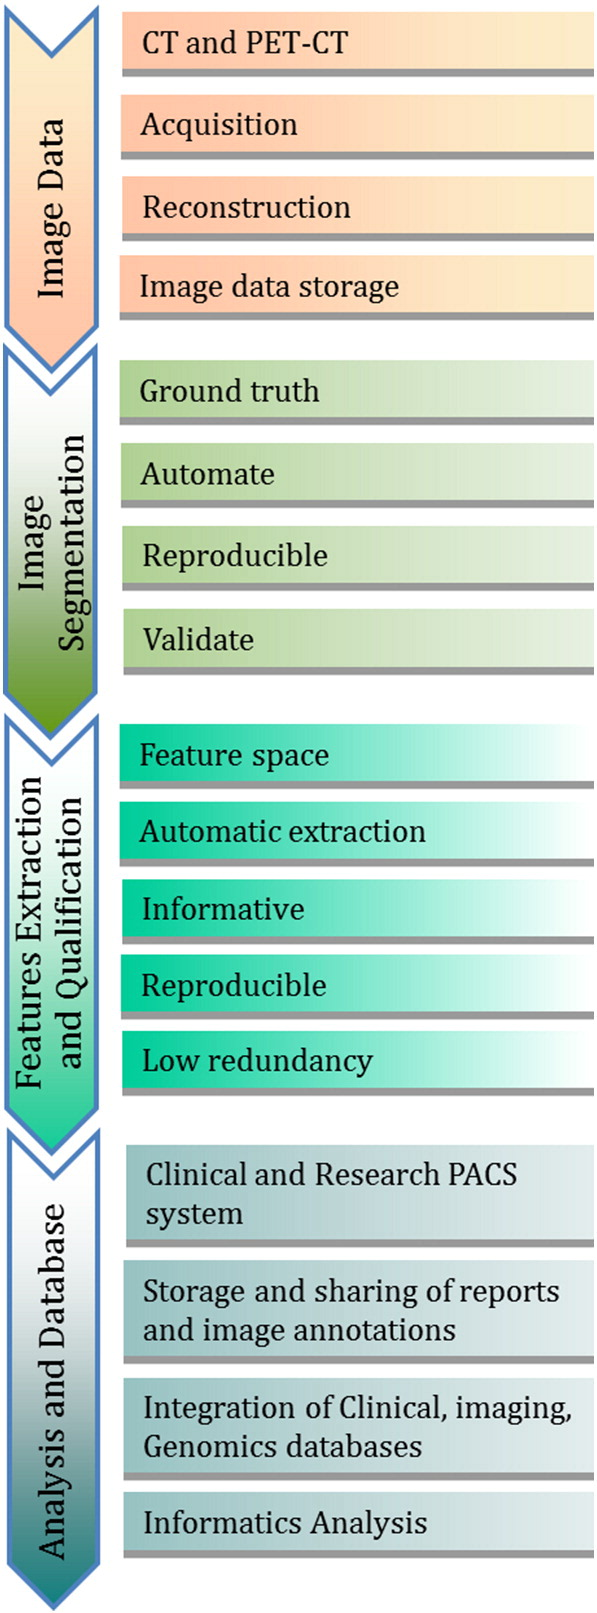
\includegraphics[height=0.8\textwidth,angle=-90]{images/radiomics_pipeline.jpg}
\caption{\small{Representation of the radiomics pipeline from\cite{kumar2012radiomics}.Each step, from right to left, is described by its fundamental characteristics.}}\label{fig:radiomics_pipeline}
\end{center}
\end{figure}


\subsubsection{Image acquisition}

Image acquisition is the step performed during clinical routine. 
Standard protocols have to be introduced in order to control the variability, already present during acquisition. 
This variability could involve image quality in terms of spatial resolution or dynamic range, patient positioning and image reconstruction.Image acquisition is highly time consuming, considering the huge amount of data needed by radiomics to overcome heterogeneities coming from the imaging process \cite{kumar2012radiomics}.

\subsubsection{Image segmentation}

Segmentation is the first step of the analysis after data acquisition.
Correct medical image segmentation is fundamental in order to improve algorithms accuracy and select precise region of interest (ROIs) for the subsequent steps \cite{biondi2021classification}.
Optimal results in image segmentation are often reached thanks to computer-aided techniques. 
Manual delineation of ROIs is often not feasible for analysis due to the presence of a non-negligible observer bias that could affect radiomic features which are very sensitive to inter- or intra-observer variability during the definition of the ROI.
Moreover, manual segmentation could be  highly time consuming, especially for very large dasets \cite{van2020radiomics-guide}.

\subsubsection{Feature extraction}

After the ROI definition there are several features that can be extracted. 
A list of the most used radiomic features \cite{van2020radiomics-guide} includes: \begin{itemize}
    \item histogram intensity-based features;
    \item shape or texture features;
    \item transform-based features;
    \item radial features.
\end{itemize}   
Large number of data can be extracted from images, thus  feature selection and dimensionality reduction techniques are sometimes used to select hierarchically  the most important ones to analyze.

\subsubsection{Data analysis}

The step of data analysis incorporates numerous techniques to evaluate the extracted features: each statistical or artificial intelligence technique must be tested on data and fine-tuned according to the aim of the study.
This last phase could even include the creation of public datasets avoiding the sharing of identified imaging data. 
The privacy concern is an important factor when the study is performed on medical data.
The creation of public dataset must take into consideration to share non-identifying data.


\subsection{Digital images application}

The most common image sources for radiomics are Magnetic Resonance Imaging (MRI), Positron Emission Tomography (PET) and  Computed Tomography (CT). 
They are standardized medical imaging techniques with well known protocols, therefore they fit perfectly for the image acquisition requirements.

However, the fast radiomics development, starting from basic research, is taking place also in clinical researches as well as daily clinical practices \cite{gillies2016radiomics-more-than-images}. 
The clinical practice is composed by medical examination (MRI, PET, CT) but also by routine visits which are not yet covered by the radiomic field in terms of research.
Clinicians could could need to take record of the ongoing treatment in chronic patients.
Therefore a need to acquire images for daily practice, beyond standard examination, arises.
Smartphones, with their digital cameras, could represent the solution to this problem as a non-standard acquisition device able to collect clinical images in daily practice.

In this work Natural ligth-reflected images acquired by smartphone digital cameras are used as starting data for the radiomic pipeline. Such data are non standardized in terms of luminosiy, acquisition distance and focus, but can still be considered relevant data carriers useful for image segmentation and feature extraction.

%some consideration about the preprocessing data?
Some pre-processing techniques were considered in order to uniformly adjust the dataset in term of brightness and contrast.
The involved trials  were Gamma correction and Contrast Limited Adaptive Histogram Equalization (CLAHE); these techniques were able to improve performances in some portion of the dataset but decreased the quality of  results on other images.
Thus it was chosen not to apply any pre-processing procedures, considering that we should specify single transformations to each image in the dataset, resulting in a non replicable pipeline.
Moreover, the non standard characteristics of the dataset is enforcing our belief on the robustness of the proposed method.


\end{document}